%%
%% sample document for AAMAS'19 conference
%%
%% modified from sample-sigconf.tex
%%
%% see ACM instructions acmguide.pdf
%%
%% AAMAS-specific questions? F.A.Oliehoek@tudelft.nl
%%

%% Additional stuff to fix .eps image files
\pdfminorversion=7
\documentclass[sigconf]{aamas}  % do not change this line!
%% your usepackages here, for example:
\usepackage{booktabs}

%% do not change the following lines
\setcopyright{ifaamas}  % do not change this line!
\acmDOI{doi}  % do noadat change this line!
\acmISBN{}  % do not change this line!
\acmConference[AAMAS'20]{Proc.\@ of the 19th International Conference on Autonomous Agents and Multiagent Systems (AAMAS 2020), B.~An, N.~Yorke-Smith, A.~El~Fallah~Seghrouchni, G.~Sukthankar (eds.)}{May 2020}{Auckland, New Zealand}  % do not change this line!
\acmYear{2020}  % do not change this line!
\copyrightyear{2020}  % do not change this line!
\acmPrice{}  % do not change this line!


%% the rest of your preamble here


%%%%%%%%%%%%%%%%%%%%%%%%%%%%%%%%%%%%%%%%%%%%%%%%%%%%%%%%%%%%%%%%%%%%%%%%%%%%%%%%%%%%%%%%%%%%%%%%%%%%%%%%%

\begin{document}

\title{Auctions for Allocation of Elastic Resources in Cloud Computing}  % put your title here!
%\titlenote{Produces the permission block, and copyright information}

% AAMAS: as appropriate, uncomment one subtitle line; check the CFP
%\subtitle{Extended Abstract}
%\subtitle{Industrial Applications Track}
%\subtitle{Socially Interactive Agents Track}
%\subtitle{Blue Sky Ideas Track}
%\subtitle{Engineering Multiagent Systems Track}
%\subtitle{Robotics Track}
%\subtitle{JAAMAS Track}
%\subtitle{Doctoral Mentoring Program}

%\subtitlenote{The full version of the author's guide is available as \texttt{acmart.pdf} document}


% AAMAS: submissions are anonymous for most tracks
\author{Paper \#XXX}  % put your paper number here!

%% example of author block for camera ready version of accepted papers: don't use for anonymous submissions
%
%\author{Ben Trovato}
%\authornote{Dr.~Trovato insisted his name be first.}
%\orcid{1234-5678-9012}
%\affiliation{%
%  \institution{Institute for Clarity in Documentation}
%  \streetaddress{P.O. Box 1212}
%  \city{Dublin}
%  \state{Ohio}
%  \postcode{43017-6221}
%}
%\email{trovato@corporation.com}
%
%\author{G.K.M. Tobin}
%\authornote{The secretary disavows any knowledge of this author's actions.}
%\affiliation{%
%  \institution{Institute for Clarity in Documentation}
%  \streetaddress{P.O. Box 1212}
%  \city{Dublin}
%  \state{Ohio}
%  \postcode{43017-6221}
%}
%\email{webmaster@marysville-ohio.com}
%
%\author{Lars Th{\o}rv{\"a}ld}
%\authornote{This author is the
%  one who did all the really hard work.}
%\affiliation{%
%  \institution{The Th{\o}rv{\"a}ld Group}
%  \streetaddress{1 Th{\o}rv{\"a}ld Circle}
%  \city{Hekla}
%  \country{Iceland}}
%\email{larst@affiliation.org}
%
%\author{Valerie B\'eranger}
%\affiliation{%
%  \institution{Inria Paris-Rocquencourt}
%  \city{Rocquencourt}
%  \country{France}
%}
%\author{Aparna Patel}
%\affiliation{%
% \institution{Rajiv Gandhi University}
% \streetaddress{Rono-Hills}
% \city{Doimukh}
% \state{Arunachal Pradesh}
% \country{India}}
%\author{Huifen Chan}
%\affiliation{%
%  \institution{Tsinghua University}
%  \streetaddress{30 Shuangqing Rd}
%  \city{Haidian Qu}
%  \state{Beijing Shi}
%  \country{China}
%}
%
%\author{Charles Palmer}
%\affiliation{%
%  \institution{Palmer Research Laboratories}
%  \streetaddress{8600 Datapoint Drive}
%  \city{San Antonio}
%  \state{Texas}
%  \postcode{78229}}
%\email{cpalmer@prl.com}
%
%\author{John Smith}
%\affiliation{\institution{The Th{\o}rv{\"a}ld Group}}
%\email{jsmith@affiliation.org}
%
%\author{Julius P.~Kumquat}
%\affiliation{\institution{The Kumquat Consortium}}
%\email{jpkumquat@consortium.net}
%
%% The example's default list of authors is too long for headers
%\renewcommand{\shortauthors}{B. Trovato et al.}


\begin{abstract}  % put your abstract here!
Abstract goes here
\end{abstract}


% AAMAS: the ACM CCS are not needed within AAMAS papers
%%
%% The code below should be generated by the tool at
%% http://dl.acm.org/ccs.cfm
%% Please copy and paste the code instead of the example below.
%%
%\begin{CCSXML}
%<ccs2012>
% <concept>
%  <concept_id>10010520.10010553.10010562</concept_id>
%  <concept_desc>Computer systems organization~Embedded systems</concept_desc>
%  <concept_significance>500</concept_significance>
% </concept>
% <concept>
%  <concept_id>10010520.10010575.10010755</concept_id>
%  <concept_desc>Computer systems organization~Redundancy</concept_desc>
%  <concept_significance>300</concept_significance>
% </concept>
% <concept>
%  <concept_id>10010520.10010553.10010554</concept_id>
%  <concept_desc>Computer systems organization~Robotics</concept_desc>
%  <concept_significance>100</concept_significance>
% </concept>
% <concept>
%  <concept_id>10003033.10003083.10003095</concept_id>
%  <concept_desc>Networks~Network reliability</concept_desc>
%  <concept_significance>100</concept_significance>
% </concept>
%</ccs2012>
%\end{CCSXML}
%
%\ccsdesc[500]{Computer systems organization~Embedded systems}
%\ccsdesc[300]{Computer systems organization~Redundancy}
%\ccsdesc{Computer systems organization~Robotics}
%\ccsdesc[100]{Networks~Network reliability}


\keywords{Edge clouds, elastic resources, auctions.}  % put your semicolon-separated keywords here!

\maketitle

%% start of main body of paper

\section{Introduction}
In the last years, cloud computing~\cite{} has become a very popular solution to run data-intensive applications remotely.
The importance of running different highly-computational tasks from a remote entity became even more popular with the
emerging technology of \emph{mobile edge computing}, which enables mobile users to run delay-sensitive computationally-intensive
tasks from the edge of mobile networks at small data-centers, known as \emph{edge clouds}.

These kinds of settings are very important for military tactical network where personal on the ground do not have the
capability's to run task that a server could. The application of this could be analysis of video from troops on the ground,
surveillance footage from UAVs or data analysis of captured enemy electronics. To do this, serveral types of resource
of the server and the task are considered: the communication bandwidth, computational and data storage / memory.
These task will also come with different important depend on who is requesting it and what the task will achieve.
In this work we demonstrate, a centralised greedy algorithm to maximise social welfare and two auction algorithms
with one centralised and the other an decentalised iterative auction. \\

%% Fidan text
%% These kind of settings are very important for \emph{military tactical networks}, where different entities need to run tasks
%% at the servers. These entities can be for instance soldiers hunting for terrorists or navy troops in a surveillance mission,
%% generals in a command center, or aircrafts or drones in a surveillance mission or performing air strikes. There are several
%% types of the resources these tasks need, such as: the communication bandwidth, computational and data storage resources.
%% When accomplished, different tasks carry different utility values to its entities. This will depend on the importance of
%% the task and also who is asking for it. E.g., a general's task has a higher utility than a major's. \\

In previous work, user would request a fix amount of resource that would be used for process the task however this can
create a bottleneck with certain resources particular with small servers used in edge cloud computing. In this work,
task will instead request the total resources required to process the task allowing the cloud provider to distribute
it's resources more efficiently to it's task due to being aware of it's tasks requirements.\\


%% Fidan Text
%% In this work, we look at a static (one-shot problem) formulation of assigning the tasks to the servers and allocating
%% optimally the resources (bandwidth, computation, and storage) to these tasks. Assuming the resources are limited, there
%% will be tasks that cannot be served. Also, there is a deadline associated with every task. So, the idea is to decide
%% which tasks to serve, to which server they are to be assigned and what amount of the resources they need to get, in order
%% to maximize the sum of the utilities over all the tasks in that moment. The approach we follow is based on auction-based techniques. \\


%\begin{itemize}
%    \item Related works
%    \item Resource allocation in cloud computing
%    \item Market based allocation
%    \item New Problem case
%\end{itemize}

\section{Related work}
In~\cite{vaji_infocom}, the authors consider the servers to be edge clouds responsible for both deciding where to place
the code/data needed to run a specific task, and also for scheduling different tasks to different edge clouds.
The goal there is to maximize the average rate of successfully accomplished tasks over time. The resources provided
by different edge clouds are heterogeneous and there is a monetary constraint for every task.

\section{System Model}
A sketch of the system is illustrated in Fig.~\ref{system_model}.
We assume that in the system there are $I$ servers, which could be edge clouds, and could be accessed either through base stations or WiFi AP.
Servers have different types of resources, such as: storage for the code/data needed to run a task, computation capacity
in terms of CPU cycles needed to run a task, and communication capacity to receive the request by a task and to send
back the results after the latter is executed. We assume that the servers are heterogeneous in all their characteristics.
We denote the storage capacity of server $i$ with $S_i$, computation capacity with $W_i$, whereas the communication capacity with $R_i$.

There are $J$ different tasks (jobs)\footnote{In this paper, we will use the notions job and task interchangeably.}
from different entities that need to be run on those servers. Running any of these tasks on the server requires storing
the appropriate code/data on the same server. These could be for example images of objects or CNN layers in identification tasks.
The size of task $j$ is denoted as $s_j$. A task also requires some CPU cycles from the server. This is denoted as $w_j$,
and is expressed in the total number of flops. A related parameter to this is the rate at which the number of flops are
assigned from the server per unit of time. We denote this as $w_{i,j}$, and its unit is Mflops/s.
Finally, after the task is run and the results obtained, the latter need to be sent back to the user.
The size of these results is denoted with $r_j$, and the rate at which they are sent from server $i$
(if the task was executed there) to the user is $r_{i,j}$. As opposed to the storage requirement of the task $s_j$ that
is \emph{strict}, the computation and communication parameters $w_{i,j}$ and $r_{i,j}$ are \emph{elastic}, i.e., the job
can be run under different values. The values of these parameters would be constrained by the deadline $D_j$ that any task
is assigned. It is the maximum time the time is allowed to ``spend'' in the system. If the task is executed completely
within that time interval by any of the servers, then the task gets the full utility $U_j$, which is specific for any task.
In case the deadline is not met, then the utility is 0. So, we have \emph{all} or \emph{nothing} task execution scheme.
It should also be mentioned that since the resources are finite, each task can be assigned to at most one server, and once
assigned it cannot switch to another server.

In this paper, we consider the static case scenario, where all jobs arrive at the same time at the start of the program.
The dynamic case (where task arrive over time) is beyond the scope of this paper. This is no task preemption as all jobs
run concurrently and so cant be stopped. We assume that every task will request at least as much resources as required to run
as any program would fail if resources were under reported.

% In this paper, we are considering the static case scenario, i.e., we look at the problem as a \emph{single shot}.
% Considering the dynamic case (as the task arrive in the system and leave after (not) being served) is beyond the scope
% of this paper. There is no task preemption. Also, we assume that every task does(not) reveal to the servers its utility,
% and (but only) its storage and computation requirement, as well as the deadline. Based on all these information, the
% servers will decide which tasks to receive and how much of the elastic resources they would allocate to the tasks they admit.
% These values will the outcomes of the following optimization problem:

% With the addition of a deadline with the job, this allows for the flexibility of the resources allocated by a server.
%% Each job ($j$) has fixed resource requirements: storage ($s_j$), computation ($w_j$) and results data ($r_j$) with a
%% deadline ($d_j$) and internal value ($v_j$). The server will allocation resources: loading speed ($s^{'}_j$),
%% compute speed ($w^{'}_j$) and sending speed ($r^{'}_j$) so that the job deadline constraint holds (equation \ref{deadline_constraint}). \\

\begin{align}
    \max & \sum^J_j U_j (\sum^I_i x_{i,j})\label{eq:objective}\\
    \mbox{s.t.} \\
    & \sum_{j=1}^{J}s_j x_{i,j}\leq S_i, &~ \forall i=1,\ldots, I,\label{eq:storage_constraint}\\
    &\sum_{j=1}^{J}w_jx_{i,j}\leq W_i, &~ \forall i=1,\ldots, I,\label{eq:computation_constraint}\\
    &\sum^J_j (r_{i,j} + s_{i,j}) x_{i,j} \leq R_i, &~ \forall i=1,\ldots I,\label{eq:communication_constraint}\\
    & \frac{s_j}{s_{i,j}} + \frac{w_j}{w_{i,j}} + \frac{r_j}{r_{i,j}} \leq \frac{D_j}{x_{i,j}}, &~ \forall{i=1,\ldots,I, j=1,\ldots,J},\label{eq:deadline}\\
    & s_{i,j}>0, &~ \forall{i=1,\ldots,I, j=1,\ldots,J},\label{eq:1}\\
    & w_{i,j}>0, &~ \forall{i=1,\ldots,I, j=1,\ldots,J},\label{eq:2}\\
    & r_{i,j}>0, &~ \forall{i=1,\ldots,I, j=1,\ldots,J},\label{eq:3}\\
    & \sum_{i=1}^{I}x_{i,j}\leq 1, &~ \forall j=1,\ldots J,\label{eq:one}\\
    & x_{i,j} \in \{0,1\}, &~ \forall{i=1,\ldots,I, j=1,\ldots,J}\label{eq:x}.
\end{align}

The objective (Eq.(\ref{eq:objective})) is to maximize the total utility over all tasks. Task $j$ will receive the full r
eward $U_j$ only if the task is executed entirely and the results are obtained within the deadline for that task.
Constraint (Eq.(\ref{eq:storage_constraint})) relates to the finite storage capacity of every server to store code/data
to run tasks. The finite computation capacity of every server is expressed through Eq.(\ref{eq:computation_constraint}),
whereas Eq.(\ref{eq:communication_constraint}) denotes the constraint on the communication capacity of the servers.
The communication bandwidth comprises of two parts: to send the data/code or request to the server, and to get the results
back to the user. Constraint Eq.(\ref{eq:deadline}) is the deadline associated with every task, where the total time
of task in the system is the sum of the time to send the request and code/data to the server, time to run the task, and
the time it takes the server to send all the results to the user. The rates at which the code is sent, run and the results
are sent back are all non-negative (Eqs.(\ref{eq:1})-(\ref{eq:3})). Further, every task is served by at most one server
(Eq.(\ref{eq:one})). Finally, a task is either served or not. Hence, the binary nature of $x_{i,j}$ (Eq.(\ref{eq:x})).

\textbf{NP-hardness:} This optimization problem is a more general case of the ``regular'' knapsack problem, which is
known to be NP-hard~\cite{}. As a result, this is an NP-hard problem. In the next section, we propose a heuristic,
with a performance guarantee of $\frac{1}{n}$.

\section{Flexible Resource Allocation Mechanisms}
Due to the flexibility of the amount of resource allocated to each task, this has meant that Dynamic Programming~\cite{}
and Bin Packing algorithms for Multiple Knapsack Problems~\cite{} cant to use as they require the weights to be fixed.
Non-linear integer programming is possible to use to solve this problem however the problems hugely intractable with
larger model sizes then 15 jobs and 3 servers. %% Probably wants to be removed

Due to the flexibility of the resource's allocated, therefore making the amounts unknown before allocation so the
traditional algorithms for solving knapsack problems, Dynamic programming, Relaxations cant work. Therefore iterative methods
for allocating jobs to servers must be used as once a job is allocated then its resource reuqirements can then we considered
fixed and other jobs can be allocated based on this allocation.

\subsection{Greedy Mechanism}
Greedy mechanism is a three stage algorithm where the jobs are ranked used a value density function. Then each jobs
from the sorted job ranks are assigned to a server using a server selection function and then the resource are allocated
to the

\subsection{Decentralised Iterative Auction Mechanism}
The addition of the deadline constraint allows for cooperation between players to be incentived as to balance the
requests for resources allowing more jobs to be allocated or for a small price. Following the VCG mechanism, we develop
an auction where job prices are calculate on an individual server bases with the price being the difference in revenue when the job runs.

If we find the value of an allocation where a job must be included and the value of the job not included then the
difference is the value of the job on the server, to increase the price we add $\epsilon$.

Each server solves the linear programming below that is the same as the problem case except with the server resource
constraints modified to include the new job (k) without the allocation variable.
\begin{align}
    \sum^J_j S_j x_{ij} + S_k \leq S_i && \forall i = 1,\dots,I; j = 1,\dots,J \\
    \sum^J_j w_j x_{ij} + w_k \leq S_i && \forall i = 1,\dots,I; j = 1,\dots,J \\
    \sum^J_j (r_j + s_j) x_{ij} + (r_k + s_k) \leq S_i && \forall i = 1,\dots,I; j = 1,\dots,J
\end{align}

\section{Empirical Evaluation}
\begin{figure*}
    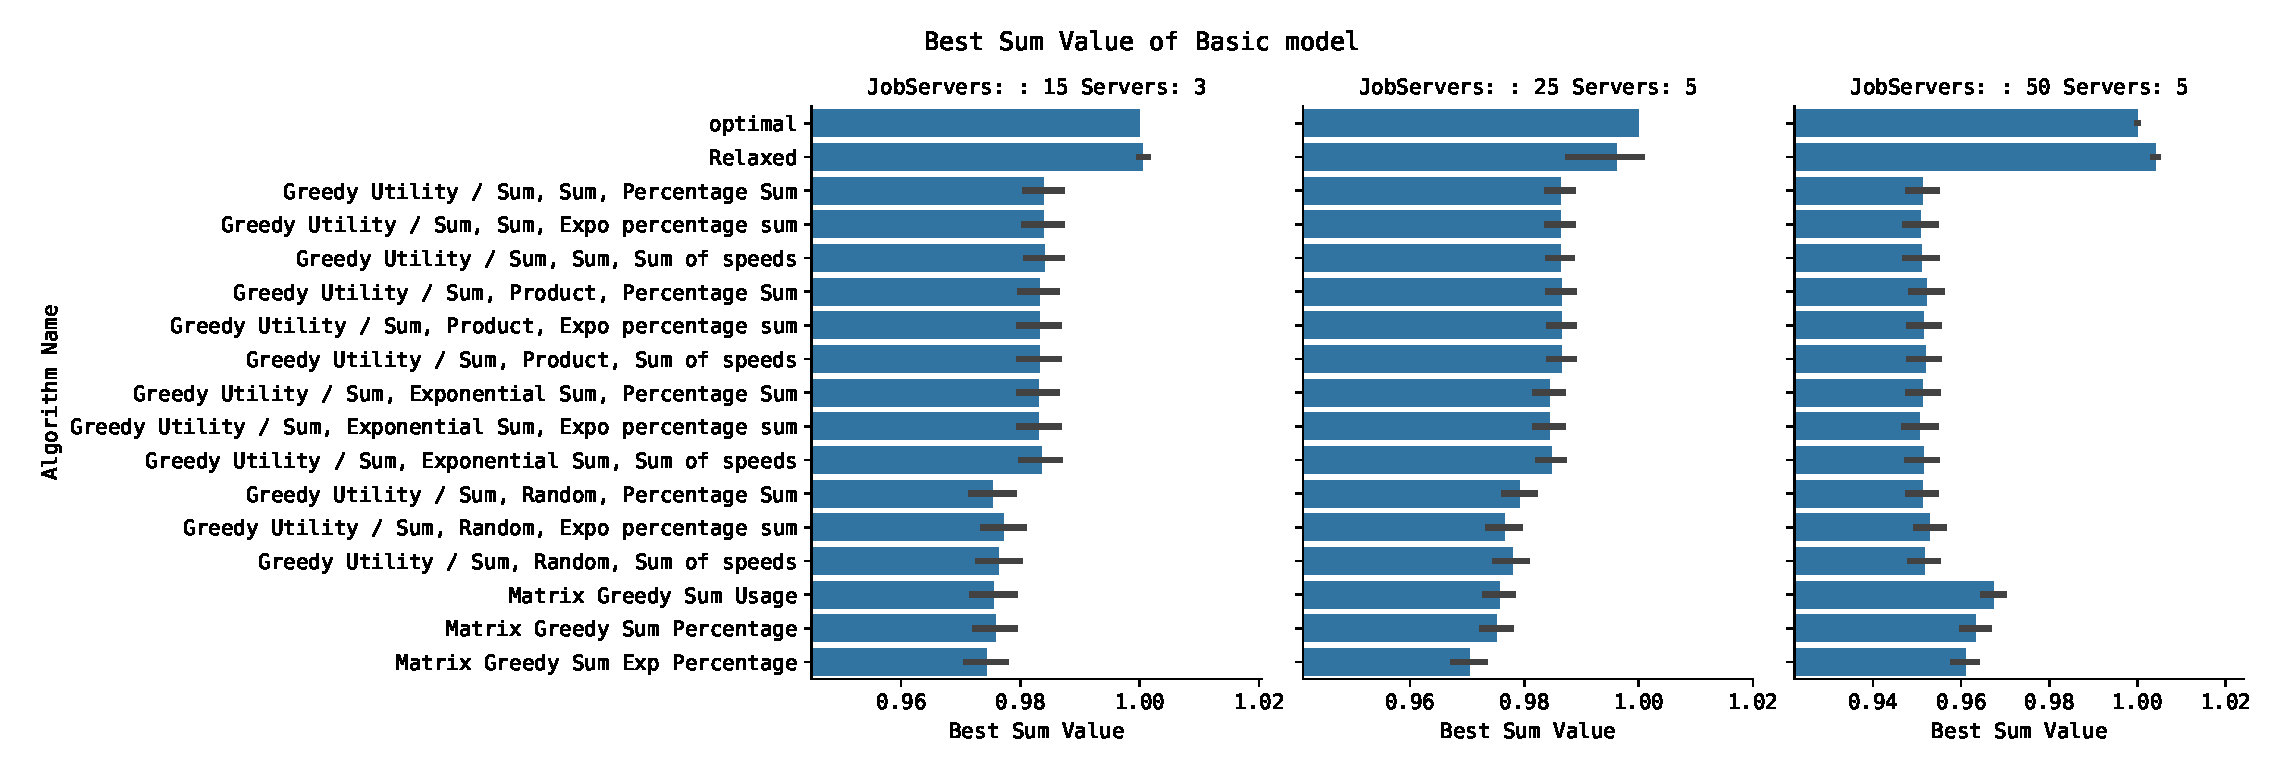
\includegraphics[width=\linewidth]{../testing/figures/greedy/eps/optimal_greedy_test_basic_best_sum_value.eps}
    \caption{Greedy algorithms with basic model measuring the sum of values}
\end{figure*}
\begin{figure*}
    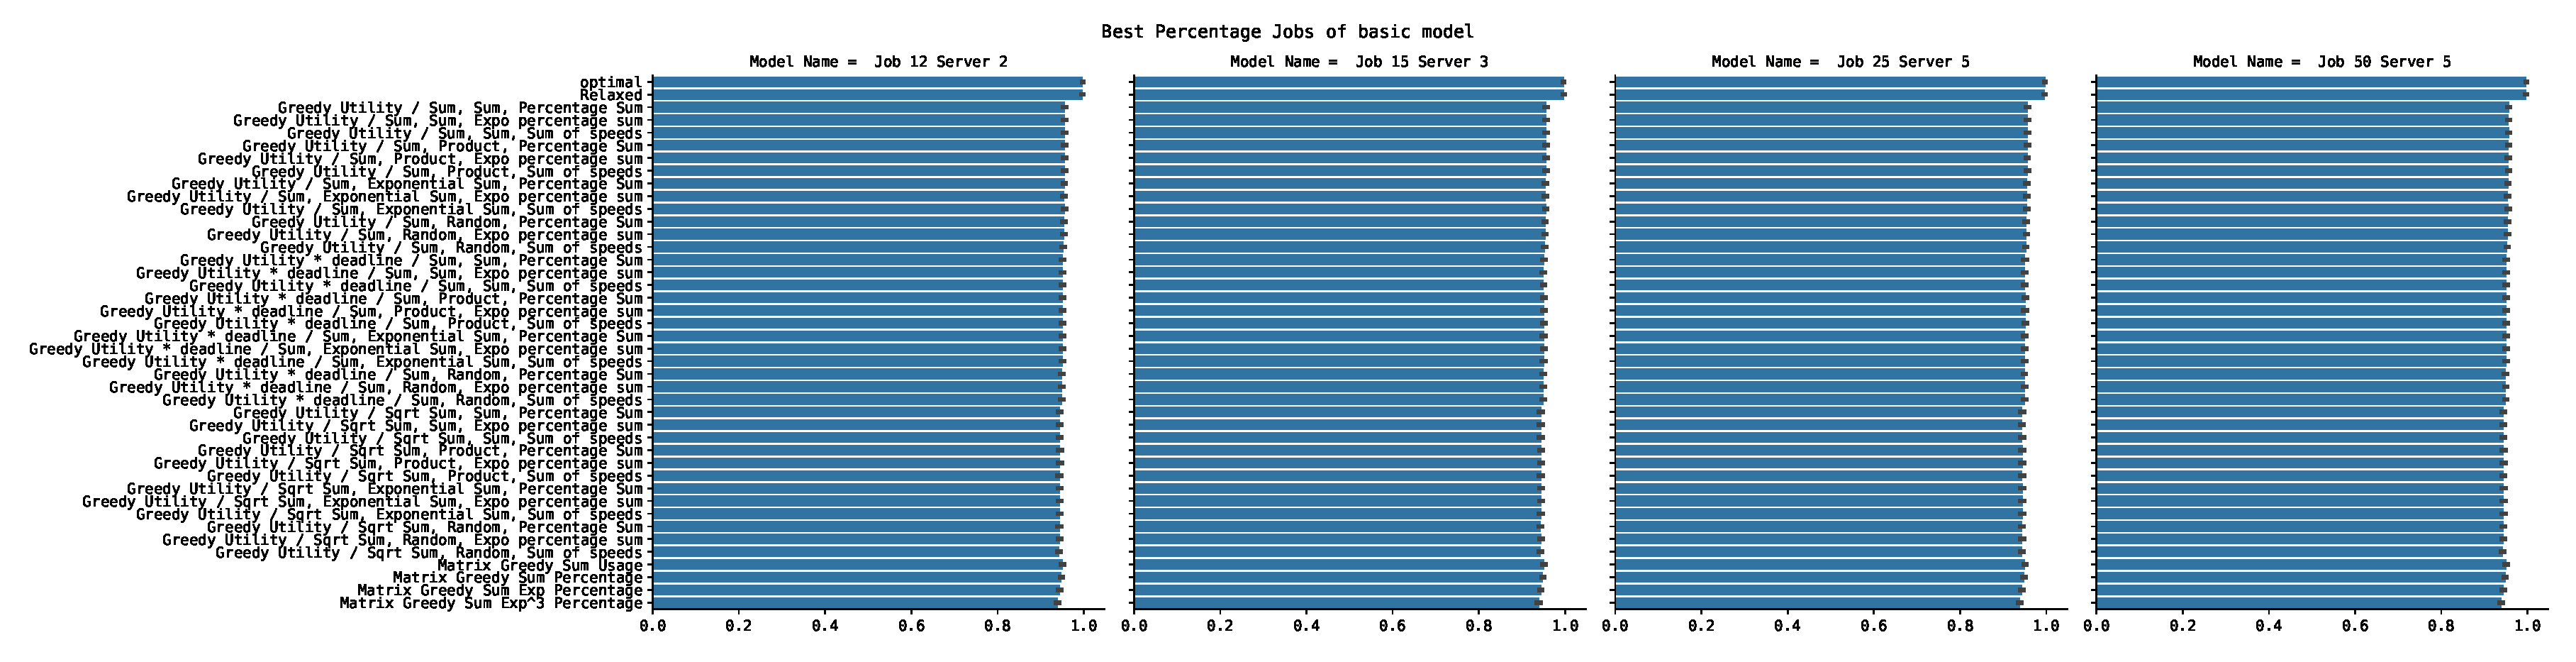
\includegraphics[width=\linewidth]{../testing/figures/greedy/eps//optimal_greedy_test_basic_best_percentage_jobs.eps}
    \caption{Greedy algorithms with basic model measuring the percentage of jobs allocated}
\end{figure*}
\begin{figure*}
    \includegraphics[width=\linewidth]{../testing/figures/greedy/eps//optimal_greedy_test_big_small_a_best_sum_value.eps}
    \includegraphics[width=\linewidth]{../testing/figures/greedy/eps//optimal_greedy_test_big_small_b_best_sum_value.eps}
    \caption{Greedy algorithms with big small model measuring the sum of values}
\end{figure*}
\begin{figure*}
    \includegraphics[width=\linewidth]{../testing/figures/greedy/eps//optimal_greedy_test_big_small_a_best_percentage_jobs.eps}
    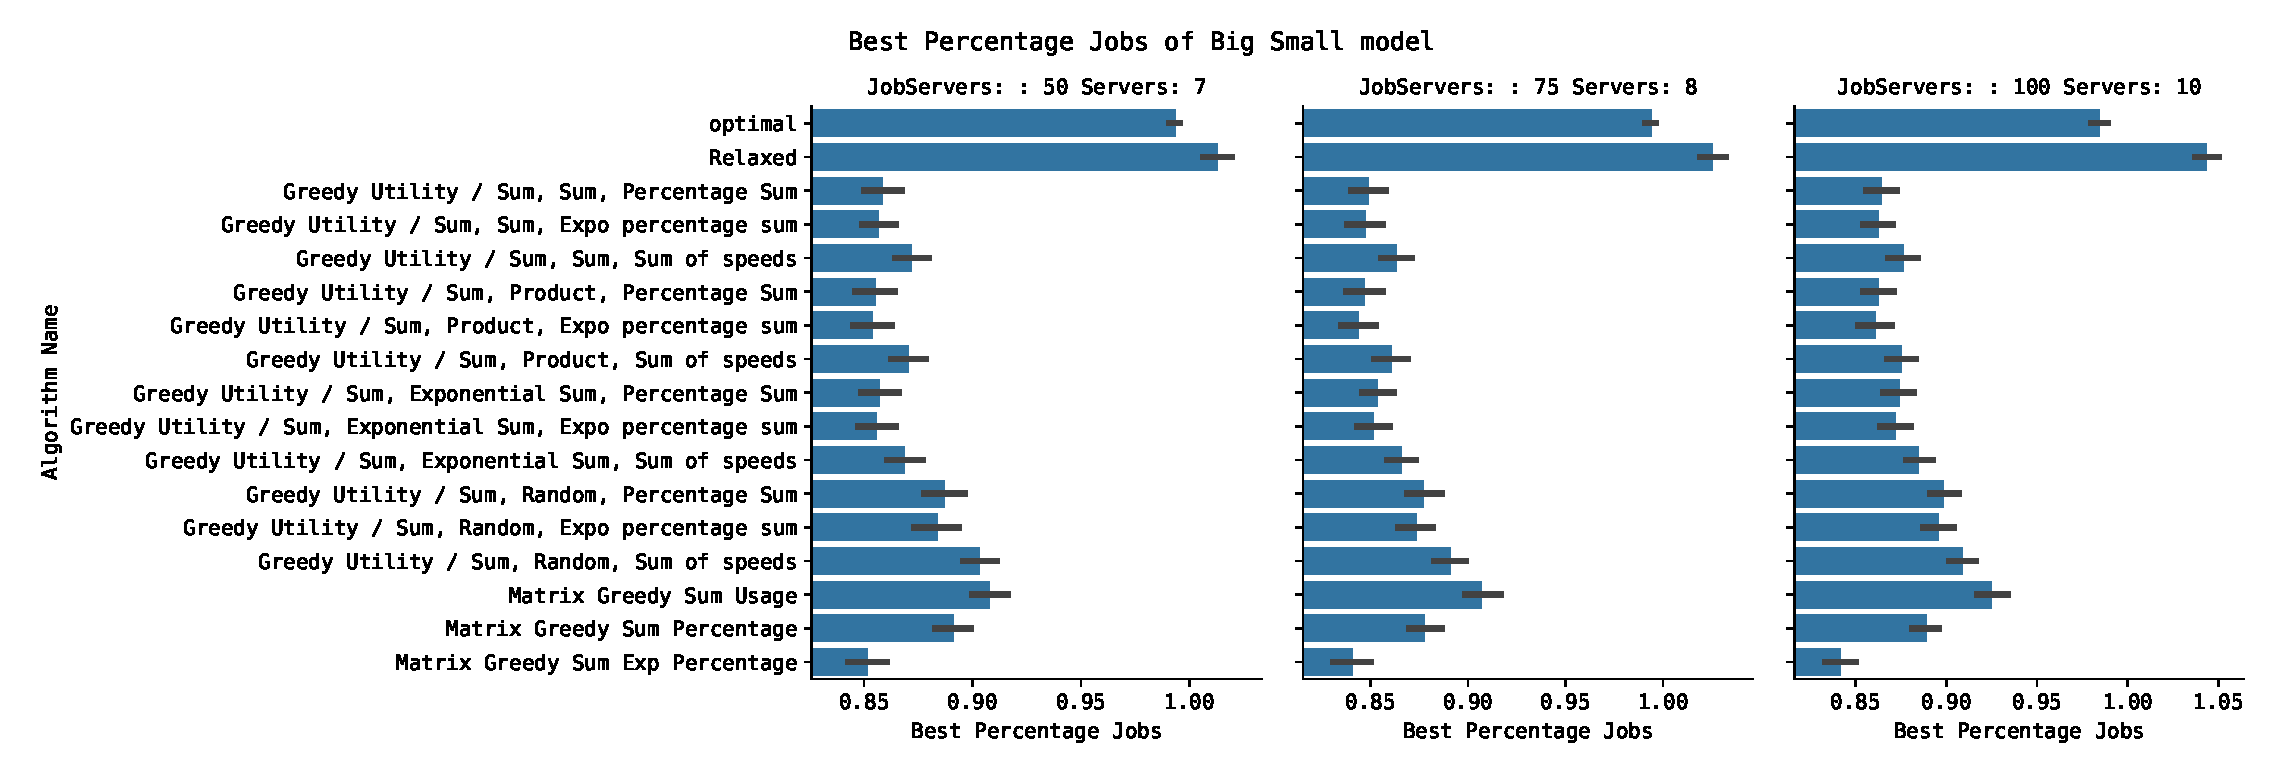
\includegraphics[width=\linewidth]{../testing/figures/greedy/eps//optimal_greedy_test_big_small_b_best_percentage_jobs.eps}
    \caption{Greedy algorithms with big small model measuring the percentage of jobs allocated}
\end{figure*}

\begin{figure*}
    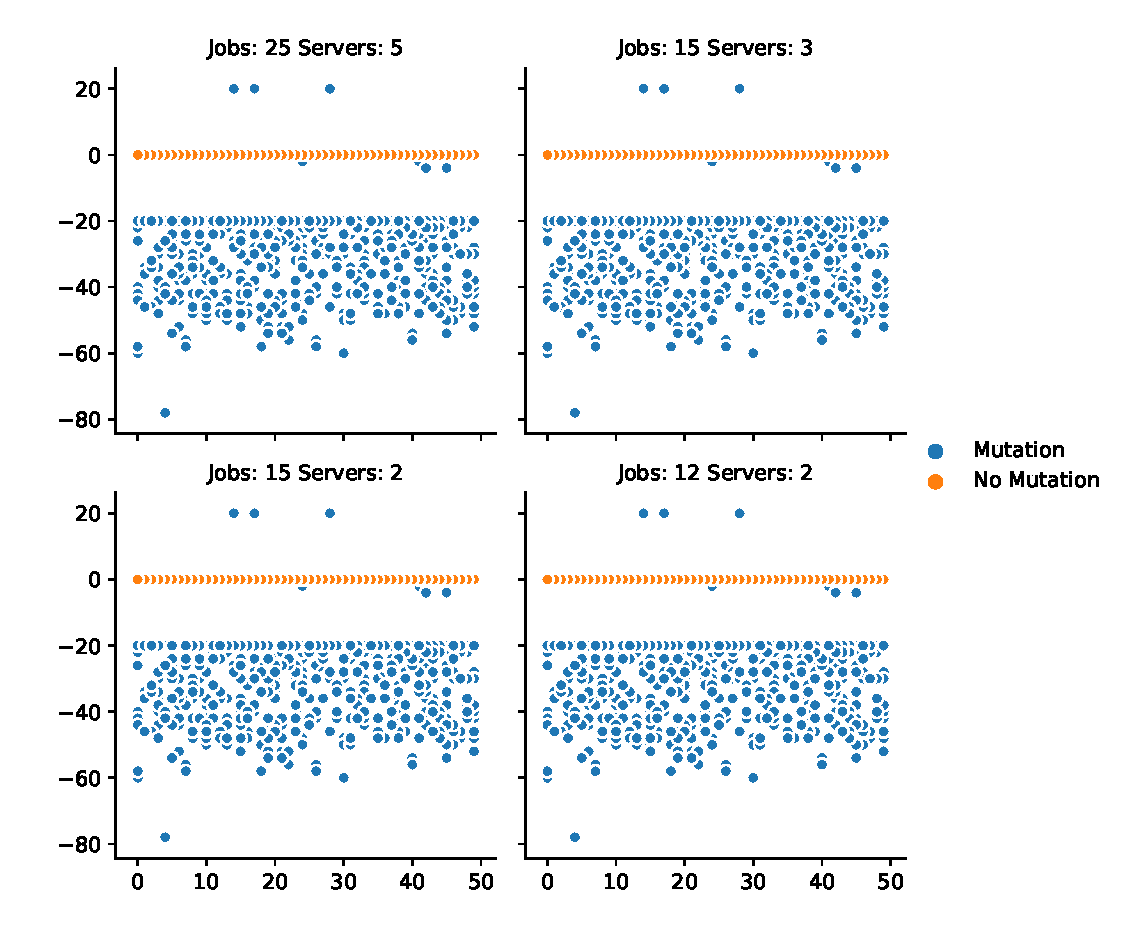
\includegraphics[width=\linewidth]{../testing/figures/auction_mutation/eps/mutate_iterative_auction_basic_mutate_difference.eps}
    \caption{Measuring the difference in price when the job is incorrectly reported}
\end{figure*}
\begin{figure*}
    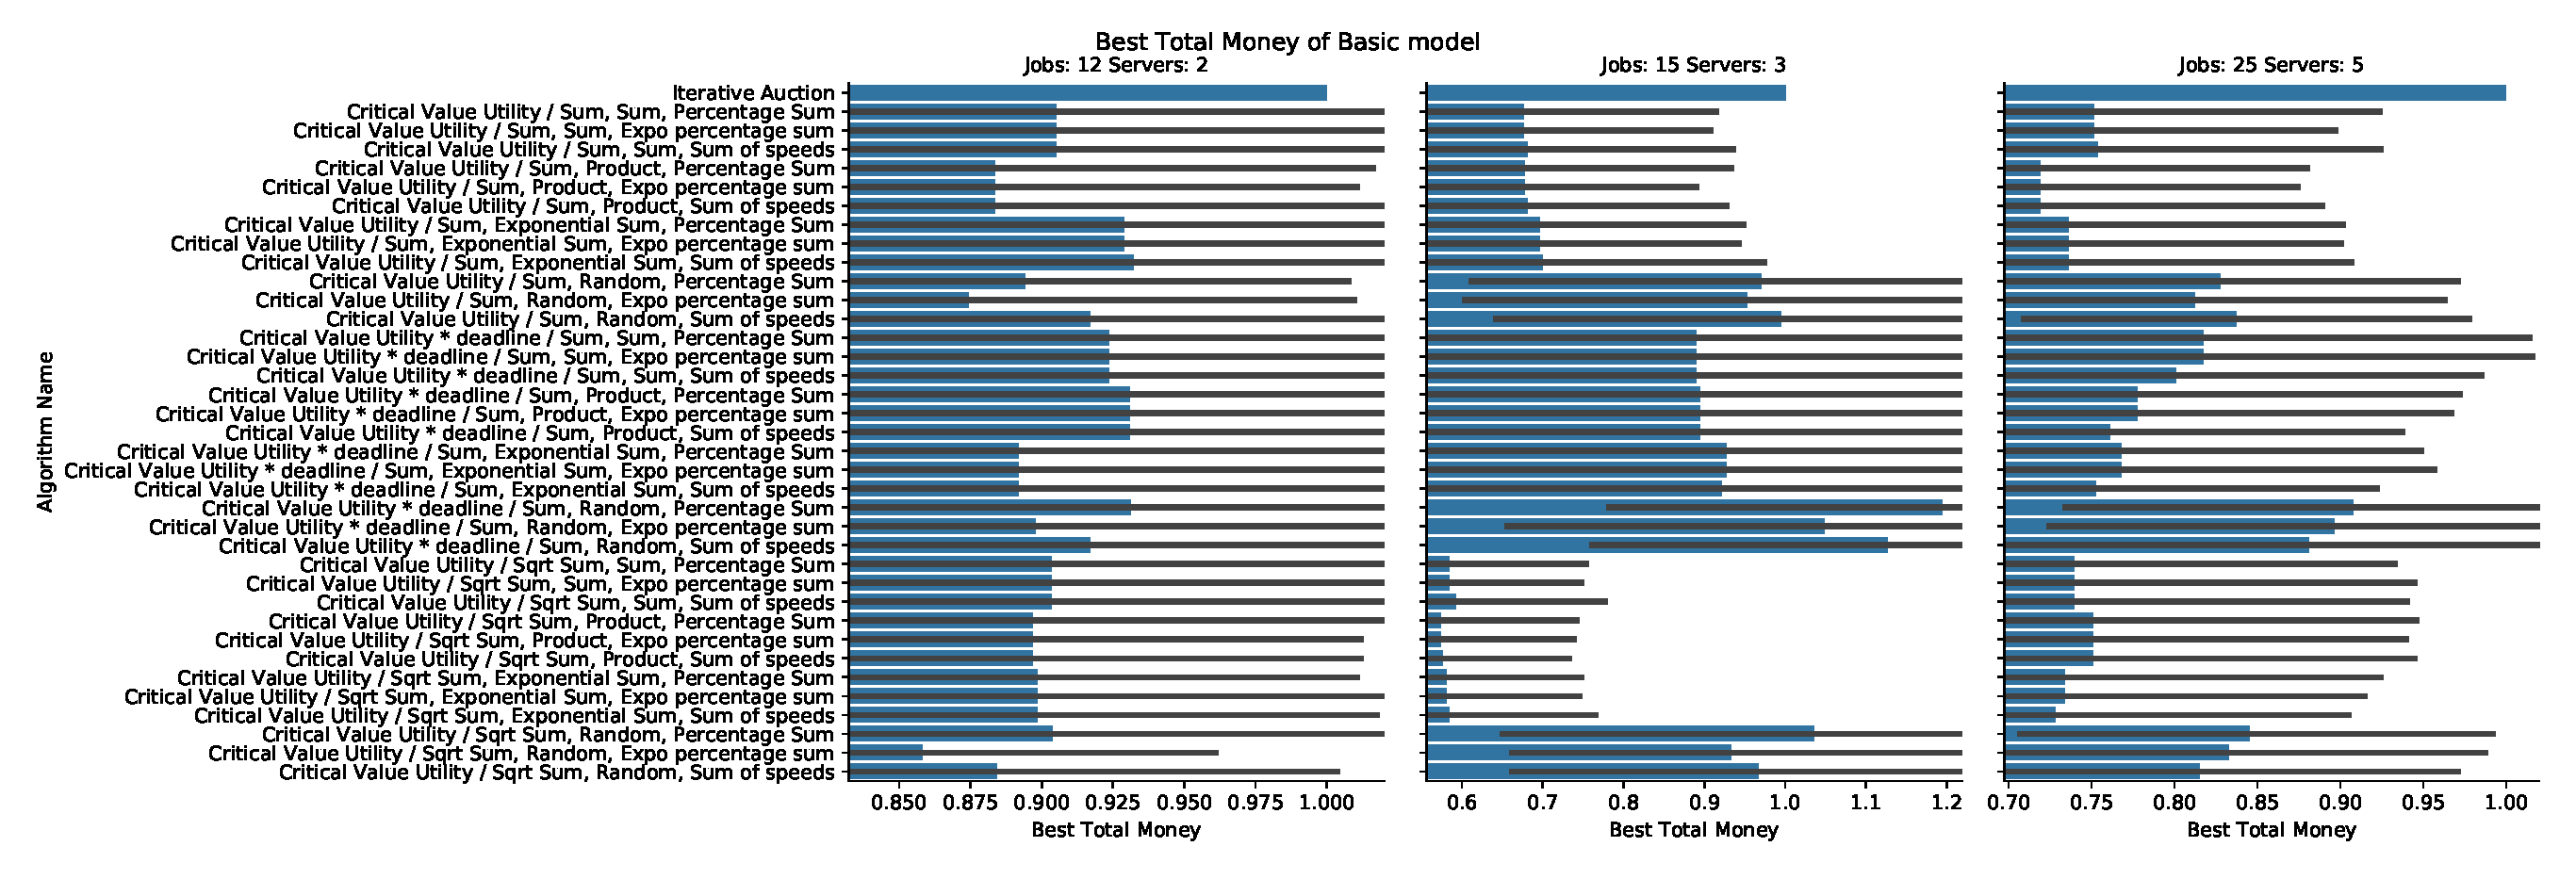
\includegraphics[width=\linewidth]{../testing/figures/critical_value/eps//critical_values_results_basic_best_total_money.eps}
    \caption{The results from the critical value algorithm total price}
\end{figure*}
\section{Conclusions and Future Work}


%%%%%%%%%%%%%%%%%%%%%%%%%%%%%%%%%%%%%%%%%%%%%%%%%%%%%%%%%%%%%%%%%%%%%%%%%%%%%%%%%%%%%%%%%%%%%%%%%%%%%%%%%
%% bibliography: see CFP for number of permitted pages

\bibliographystyle{ACM-Reference-Format}  % do not change this line!
\bibliography{bibliography}  % put name of your .bib file here

\end{document}
